\documentclass[a4paper, 14pt]{extreport} %размер бумаги устанавливаем А4, шрифт 12пунктов
\usepackage{extsizes}
\usepackage[T2A]{fontenc}
\usepackage[utf8]{inputenc}
%\usepackage{pscyr}
\usepackage{indentfirst} % отделять первую строку раздела абзацным отступом тоже
\usepackage[english,russian]{babel}
\usepackage[]{graphicx}
\usepackage[usenames,dvipsnames]{color} % названия цветов
\usepackage{amssymb,amsfonts,amsmath,amsthm,mathtext,cite,enumerate,float} %подключаем нужные пакеты расширений

%\usepackage{makecell}
\usepackage{multirow} % улучшенное форматирование таблиц
%\usepackage{ulem} % подчеркивания
%\linespread{1.3} % полуторный интервал

%\renewcommand{\caption}{\fontsize{7}{8.4pt}\selectfont Рис. \value{thefigure} }

%\usepackage{setspace}

% \onehalfspacing
%\renewcommand{\rmdefault}{ftm} % Times New Roman
\frenchspacing
\usepackage{geometry} % Меняем поля страницы

\geometry{left=2cm}% левое поле
\geometry{right=1cm}% правое поле
\geometry{top=2cm}% верхнее поле
\geometry{bottom=2cm}% нижнее поле
\graphicspath{{images/}}

%\renewcommand{\chaptertitlename}{Глава}
% Настройка вертикальных и горизонтальных отступов



\usepackage{tocloft}
\renewcommand{\cfttoctitlefont}{\hspace{0.38\textwidth} \bfseries\MakeUppercase}
\renewcommand{\cftbeforetoctitleskip}{-1em}
\renewcommand{\cftaftertoctitle}{\mbox{}\hfill \\ \mbox{}\hfill{\footnotesize Стр.}\vspace{-2.5em}}
\renewcommand{\cftchapfont}{\normalsize\bfseries \MakeUppercase{\chaptername} }
\renewcommand{\cftsecfont}{\hspace{31pt}}
\renewcommand{\cftsubsecfont}{\hspace{11pt}}
\renewcommand{\cftbeforechapskip}{1em}
\renewcommand{\cftparskip}{-1mm}
\renewcommand{\cftdotsep}{1}
\setcounter{tocdepth}{2}

\newcommand{\empline}{\mbox{}\newline}
\newcommand{\likechapterheading}[1]{
     \begin{center}
     \textbf{\MakeUppercase{#1}}
     \end{center}
     \empline}
\makeatletter
     \renewcommand{\@dotsep}{2}
     \newcommand{\l@likechapter}[2]{{\bfseries\@dottedtocline{0}{0pt}{0pt}{#1}{#2}}}
\makeatother
\newcommand{\likechapter}[1]{
     \likechapterheading{#1}
     \addcontentsline{toc}{likechapter}{\MakeUppercase{#1}}}


\usepackage[square,numbers,sort&compress]{natbib}

\renewcommand{\bibnumfmt}[1]{#1.\hfill} % нумерация источников в самом списке — через точку
\renewcommand{\bibsection}{\likechapter{Список использованных источников}} % заголовок специального раздела
\setlength{\bibsep}{0pt}


\usepackage[bf]{titlesec}

\titleformat{\chapter}[display]
     {\filcenter}
     {\bfseries {\MakeUppercase{\chaptertitlename} \thechapter}}
     {8pt}{\bfseries}

\titleformat{\section}
     {\normalsize \bfseries}
     {\thesection}
     {1em}{}

\titleformat{\subsection}
     {\normalsize \bfseries}
     {\thesubsection}
     {1em}{}
  \titlespacing*{\chapter}{0pt}{-30pt}{8pt}
\titlespacing*{\section}{\parindent}{*4}{*4}
\titlespacing*{\subsection}{\parindent}{*4}{*4}


\usepackage{listings}
%...



\begin{document}

\sloppy
%\input{diplom-title}
%%титульная страница
%\maketitle
\input{diplom-title}


\setcounter{page}{2}
\newpage
\likechapter{РЕФЕРАТ}



 Работа, 28 с., 24 рис.,  8 источников.

ПРИНЦИП УСТАНОВЛЕНИЯ, ЖЁСТКИЕ ЗАДАЧИ, МЕТОД РУНГЕ-КУТТЫ, СОБСТВЕННЫЕ ЗНАЧЕНИЯ, СПЕКТРАЛЬНЫЙ РАДИУС

Объект исследования – методы решения жёстких задач.

Цель работы – разработка вычислительного алгоритма для решения жёстких дифференциальных задач на основе принципа установления.

Методы исследования – методы численного анализа.%, методы оптимизации.

Результатом является алгоритм решения жёстких дифференциальных задач, в основе которого лежит принцип установления.

Областью применения является решение задач математической физики.

Работа выполнена при поддержке гранта БРФФИ №Ф12МВ-006.
\newpage
\renewcommand\contentsname{Содержание} 
\tableofcontents
\newpage
\likechapter{ВВЕДЕНИЕ}

Жесткие задачи исследуются примерно со второй половины 20-го века.
Однако до сих пор трудно сформулировать точное определение
жесткости. Исторически первым было определение данное Кёртиссом и
Хиршфельдером в 1952 году: {\it жесткие уравнения -- это уравнения,
для которых определенные неявные методы дают лучший результат,
обычно несравнимо более хороший чем явные методы}. Хотя это
определение не претендует на полноту и уж тем более на строгость,
оно в достаточной мере характеризует проблему: большинство явных
методов не приспособлены к решению жестких задач.

Более полным является определение данное Ламбертом: \emph{если
численный метод с ограниченной областью абсолютной устойчивости,
примененный к системе с произвольными начальными условиями вынужден
использовать на некотором интервале интегрирования величину шага,
которая черезмерно мала по отношению к гладкости точного решения на
этом интервале, тогда говорят что система является жесткой на этом
интервале}.

%Во многих источниках можно найти частные определения жесткости.
%Например, в случае линейных систем жесткой называют систему, у
%которой все действительные части собственных значений  меньше ноля.
%
%Таким образом, в случае жёстких систем, на величину шага
%интегрирования (а значит и на трудоёмкость вычислений) большее
%влияние оказывают соображения вычислительной устойчивости, а не
%точности.

% Как было сказано ранее, явные методы в большинстве своём не
% применимы для жёстких задач. Неявные же методы на жёстких задачах
% работают лучше, но требуют на каждом шаге дополнительно решения
% системы в общем случае нелинейных уравнений. Поэтому основной
% трудностью в интегрировании жестких задач неявными методами
% заключается в решении возникшей системы.

При применении неявного метода к линейной задаче возникает система
линейных уравнений, которую можно решать,  вообще говоря, любым
методом решения линейных систем. Но следует учитывать специфику:
во-первых, система как правило большой размерности, что исключает
применение прямых методов решения в силу черезмерной трудоемкости и
возможности накопления вычислительной погрешности; во-вторых, у
возникшей системы спектр как правило комплексный, что не даёт
эффективно применять итерационные процессы типа Якоби. Остаются
методы, основанные на подпространствах Крылова.

В нелинейном случае для реализации неявных методов очень часто
применяются методы ньютоновского типа. Но их применение, как
известно, также сопряжено с процедурой решения больших СЛАУ, что в
случае больших систем неприемлемо ввиду излишней трудоемкости. К
тому же, для сходимости метода Ньютона необходимо выбрать достаточно
близкое начальное приближение, что также является не самой простой
задачей.

Учитывая всё вышесказанное, хотелось бы получить алгоритм решения
жестких задач, который бы не требовал обращения матриц, был применим
в нелинейном случае, являясь одновременно простым и удобным для
реализации. Описанию такого алгоритма и посвящена данная работа.

%Ниже  изложен алгоритм реализации неявных методов для жестких задач, основанный на принципе установления.%, и некоторые соображения по его применимости.



\chapter{ТЕОРЕТИЧЕСКИЕ СВЕДЕНИЯ}
%\addcontentsline{toc}{chapter}{2 Теория}
%\refstepcounter{chapter}


% можно воспользоваться методом Rhote, суть которого заключается в дискретизации сначала по времени, а затем по пространству.
%Хотелось бы получить семейство методов, обладающих удобством реализации как у явных методов, но применимых для жёстких задач, о чём и пойдёт речь в данной работе.
\section{Линейный случай}
Рассмотрим задачу Коши для неоднородной линейной системы обыкновенных дифференциальных уравнений (ОДУ)
\begin{equation}
\begin{aligned}
\label{main_problem}
&y'(t)=Jy(t)+f(t),\\
&y(t_0)=y_0,\\
&t \in [t_0, t_0+\tau],\quad \\
&y_0\in \mathbb{R}^N,\quad
y:[t_0,t_0+\tau] \to \mathbb{R}^N,\quad\\
&J \in \mathbb{R}^N \times \mathbb{R}^N, \quad
\tau \in [0, +\infty).\\
\end{aligned}
\end{equation}
Для нахождения приближения к $y(t_0+\tau)$, $\tau >0$ проинтегрируем её произвольным $s$-стадийным неявным методом типа Рунге-Кутты (базовым методом), представленным следующей таблицей Бутчера
\begin{center}
\begin{equation}
\label{base_method}
\begin{array}{l|lll}
c_1& a_{11}& ...& a_{1s}\\
...& ...& ...& ...\\
c_s& a_{s1}& ...& a_{ss}\\
\hline
& b_1& ...& b_s\\
\end{array}
\end{equation}
\end{center}
Здесь $A=(a_{i,j})_{i,j=1}^s$ -- так называемая матрица Бутчера
базового метода. Тогда
$$ y(t_0+\tau)\thickapprox y_1=y_0+\tau\sum_{i=1}^sb_ik_i,$$
где $\{k_i\}_{i=1}^s$ находятся как решение следующей системы линейных алгебраических уравнений (СЛАУ)
$$k_i = J(y_0+\tau\sum_{j=1}^sa_{ij}k_j)+f(t_0+c_i\tau).$$
В дальнейшем будем пользоваться матричной записью этой СЛАУ:
\begin{equation}\label{system_for_solving}
\begin{aligned}
&(\tau A\otimes J-I)k+g=0,\\
&g=(g_1,g_2,..,g_s)^T, \quad g_i=f(t_0+c_i \tau)+Jy_0, \quad i=1,..,s,\\
&k=(k_1,k_2,..,k_s)^T, \quad k_i \in \mathbb{R}^N.\\
\end{aligned}
\end{equation}
Здесь $\otimes$ обозначает кронекеровское произведение матриц\cite{dekker}, по
определению которого получаем, что $$G=\tau A\otimes J-I$$ -- блочная
матрица вида
\begin{equation}
\left(
\begin{array}{llll}
-1+\tau a_{11}J& \tau a_{12}J&...&\tau a_{1s}J\\
 \tau a_{12}J&-1+\tau a_{22}J&...&\tau a_{2s}J\\
...&...&...&...\\
\tau a_{s1}J& \tau a_{s2}J&...&-1+\tau a_{ss}J\\
\end{array}
\right ).
\end{equation}


\section{Уравнение установления}
Рассмотрим вспомогательное уравнение
\begin{equation}
\label{estEquation}
k'=(\tau A\otimes J-I)k+g=Gk+g = r(k),
\end{equation}
которое в дальнейшем будем называть уравнением установления.

Очевидно, что точное решение уравнения \eqref{system_for_solving}
$k^*$ будет являться стационарным решением \eqref{estEquation}. Для
этого достаточно, чтобы спектр матрицы $G$ целиком содержался в
левой комплексной полуплоскости. Поэтому, если проинтегрировать~\eqref{estEquation}  каким-нибудь численным методом, то можно
получить приближение к решению \eqref{system_for_solving}.

Для решения \eqref{estEquation} будем использовать явный метод Рунге-Кутты, задаваемый таблицей вида
\begin{equation}
\label{auxilary_method_table}
\begin{array}{lllll}
 \alpha_{21}& & & &  \\
 \alpha_{31}&\alpha_{32} & & &  \\
 ...& ...& ...& &\\
 \alpha_{\sigma1}& \alpha_{\sigma2}&... &\alpha_{\sigma\sigma-1}&  \\
\hline
 \beta_1&\beta_2 &...&\beta_{\sigma-1}& \beta_\sigma\\
\end{array}
\end{equation}
Пусть $\omega$ - шаг по фиктивному времени. В результате получаем
итерационный процесс вида
\begin{equation}\label{ipe_gf}
\begin{aligned}
&k^{l+1}=\Phi(k^{l})\\
&\Phi(k)=k+\omega \sum_{p=1}^\sigma\beta_pK_p(k),\\
&K_p(k)=G (k +\omega\sum_{q=1}^{p-1}\alpha_{pq} K_q(k))+g.
\end{aligned}
\end{equation}
Учитывая специфику интегрирования уравнения установления \eqref{estEquation}, нужно выбрать  $\omega$, $\{\alpha_{ij}\}_{i,j=1}^{\sigma}$, $\{\beta_i\}_{i=1}^{\sigma}$.

\section{Выбор вспомогательного метода Рунге-Кутты}

Для выбора коэффициентов вспомогательного метода заметим, что процесс \eqref{ipe_gf} представим в виде
\begin{equation}
\label{ipe_spektr_form}
k^{l+1} = R_\sigma(\omega G)k^l+P(\omega, G),
\end{equation}
где $R_\sigma$ -- многочлен степени $\sigma$, называемый многочленом перехода (функцией устойчивости),  $P$ -- функция, точный вид которой несущественен в данном случае.

Известно, что многочлен перехода во многом определяет свойства
устойчивости метода интегрирования ОДУ. В нашем же случае он
определяет свойства сходимости итерационного процесса. Мы
заинтересованы в том, чтобы вспомогательный метод был устойчив на
как можно большей области. В частности, область устойчивости
$$ S = \{z \in \mathbb{C}\ :\  |R_{\sigma}(z)|<1  \}$$
должна содержать в себе  спектр матрицы $\omega G$ \cite{Faleichik_Bondar_Kyiv}.% Поэтому $\omega$ следует положить равным спектральному радиусу матрицы Якоби.

Запишем многочлен устойчивости в виде
 $$R_{\sigma}(z)=1+\sum_{j=1}^\sigma a_jz^j,$$
где $z \in \mathbb{C}$. Коэффициенты $\{a_i\}_{i=1}^\sigma$, $a_i\in \mathbb{R}$ будем выбирать таким образом, чтобы
%$$u'(h)=\lambda u(h) +\varphi(h), \quad u(t_0) = u_0$$
%Выбор метода интегрирования~(\ref{estEquation}) будем производить следующим образом: построим множитель (многочлен) перехода таким образом, чтобы его область устойчивости как можно лучше покрывала  (обозначим её $\Omega(\alpha)$, $\Omega(\alpha)=\{(\rho,\varphi):|R(\rho e^{\mathrm i\varphi})|<1\}$ )
\begin{equation}
\label{minimizeR}
F(a_1,...,a_\sigma)=\int_0^1\int_{\pi-\alpha}^{\pi+\alpha}|R_\sigma(\rho e^{\mathrm i\varphi})|^2d\varphi
d\rho\longrightarrow \min.
\end{equation}
Здесь $\alpha$ - некоторый заранее заданный угол, определяющий область устойчивости полинома $R_\sigma$ \cite{Faleichik_article},\cite{Faleichik_bondar_amade}. Вообще, $\alpha$ нужно выбирать исходя из представлений о спектре матрицы $G$, поскольку чем лучше будет приближен спектр, тем более эффективным будет метод. Параметр $\omega$ выбирается так, чтобы спектр матрицы $\omega G$ полностью содержался в области устойчивости. Для этого достаточно положить $\omega$ равным спектральному радиусу матрицы $G$. Примеры областей устойчивости полученных для значений угла $\alpha$ равных $\frac{\pi}{2}$,$\frac{\pi}{3}$,$\frac{\pi}{4}$,  $\frac{\pi}{6}$ и $\sigma = 20$ можно увидеть на рисунке \ref{domains}.
\begin{figure}
\begin{center}
\begin{tabular}{cc}
\includegraphics[height=4cm]{domain_pi_2.pdf}&\includegraphics[height=4cm]{domain_pi_3.pdf}\\
\small{  $\alpha=\frac{\pi}{2}$} & \small{ $\alpha=\frac{\pi}{3}$}\\
\includegraphics[height=4cm]{domain_pi_4.pdf}&\includegraphics[height=4cm]{domain_pi_6.pdf}\\
\small{ $\alpha=\frac{\pi}{4}$} &\small{ $\alpha=\frac{\pi}{6}$}
\end{tabular}
\caption{\small Пример областей устойчивости. }
\label{domains}
\end{center}
\end{figure}

 Метод, полученный с $\alpha = \frac{\pi}{2}$ будет применим для всех задач со спектром из левой комплексной полуплоскости, однако будет проигрывать по эффективности применимым методам с меньшими углами  (см. Рис \ref{spectr_in_regionn}).
\begin{figure}
\begin{center}
\begin{tabular}{cc}

\includegraphics[height=8cm]{spectr_in_region1.png}&\includegraphics[height=8cm]{spectr_in_region2.png}\\
\small{ a)} & \small{ б)}\\

\includegraphics[height=8cm]{spectr_in_region3.png}&\includegraphics[height=8cm]{spectr_in_region4.png}\\
\small в) &\small г)
\end{tabular}
\caption{\small Пример расположения спектра в области устойчивости вспомогательного метода: методы а, б, в применимы, причем в -- наиболее эффективный; метод г не применим }
\label{spectr_in_regionn}
\end{center}
\end{figure}

Определим коэффициенты многочлена $R_{\sigma}$(здесь и далее полагаем $a_0=1$):
\begin{multline*}|R_{\sigma}(\rho e^{\mathrm i \varphi})|^2=\mathrm{Re}(R_{\sigma}(\rho e^{\mathrm i \varphi}))^2+\mathrm{Im}(R_{\sigma}(\rho e^{\mathrm i \varphi}))^2 =\\
=(1+\sum_{j=1}^\sigma a_j\rho^j\cos(j\varphi))^2+ (\sum_{j=1}^\sigma a_j\rho^j\sin(j\varphi))^2 =\\
= 1 + \sum_{p=1}^{\sigma}\rho a_p\cos(p\varphi) + \sum_{p=1}^\sigma \sum_{q=1}^\sigma\rho^{p+q}a_pa_q\cos(p\varphi)\cos(q \varphi)+ \\
+\sum_{p=1}^\sigma \sum_{q=1}^\sigma\rho^{p+q}a_pa_q\sin(p\varphi)\sin(q \varphi) =\\
\end{multline*}
\begin{multline*}
=\left[a_pa_q\cos(p\varphi)\cos(q\varphi)+a_pa_q\sin(p\varphi)\sin(q\varphi) =\frac{1}{2}a_pa_q\cos((p-q)\varphi)  \right]=\\
=1+\sum_{p=1}^{\sigma}\rho a_p\cos(p\varphi)+
\sum_{p=1}^\sigma \sum_{q=1}^\sigma\frac{1}{2}\rho^{p+q}a_pa_q \cos((p-q)\varphi)\\
\end{multline*}
Тогда:
\begin{multline}
\label{functionalF}
F(a_1,...,a_\sigma)=\int_0^1\int_{\pi-\alpha}^{\pi+\alpha}1+\sum_{p=1}^{\sigma}\rho a_p\cos(p\varphi)+\\+
\sum_{p=1}^\sigma \sum_{q=1}^\sigma\frac{1}{2}\rho^{p+q}a_pa_q \cos((p-q)\varphi)d\varphi d\rho
\end{multline}
Чтобы найти минимум функционала~(\ref{functionalF}), необходимо найти точку, в которой $\frac{\partial F}{\partial a_j} = 0, j=1,...,\sigma$:
\begin{multline}
\label{linearSystemForRcoef}
\frac{\partial F}{\partial a_j}=\sum_{q=1}^{\sigma}a_{q}\int_{0}^{1}\int_{\pi-\alpha}^{\pi+\alpha} \rho^q \cos((q-j)\varphi)d\varphi d\rho + \int_{0}^{1}\int_{\pi-\alpha}^{\pi+\alpha} \rho \cos(j\varphi)d\varphi d\rho=0 ,\\
\quad j=1,...,\sigma.\\
\end{multline}
Решив систему уравнений~(\ref{linearSystemForRcoef}), мы и найдем искомые коэффициенты $\{a_i\}_{i=1}^\sigma$ определяющие многочлен $R(z)$.

По построенному множителю перехода восстановим таблицу явного метода, воспользовавшись способом описанным в \cite{hairer}, \cite{Faleichik_amade}: представим вспомогательный метод в виде суперпозиции двухстадийных и, возможно, одного одностадийного метода. Тогда
$$
\Phi=\Phi_{\sigma'} \circ \Phi_{\sigma'-1} \circ...\circ \Phi_{1}, \quad \sigma' = \lceil \sigma/2\rceil,
$$
что соответствует разложению $R(z)$ на множители вида $(1+\delta_m z)(1+\delta'_m z)$, $\delta_m$ и $\delta'_m$ $\in \mathbb R$ или  $\delta_m$ и $\delta'_m$ $\in \mathbb C$
и множитель  $(1+\gamma z)$, $\gamma \in \mathbb R$, появляющийся при нечётных $\sigma$.

При четных $\sigma$ все методы являются двухстадийными явными методами Рунге-Кутты:
$$\Phi_m(k) = k+\omega (\beta_{m,1}r(k)+\beta_{m,2}r(k+\omega \alpha_m r(k)),$$
где коэффициенты $\alpha_m$, $\beta_{m,1}$, $\beta_{m,2}$ удовлетворяют соотношению
$$(1+\delta_m z)(1+\delta_m'z)=1+(\beta_{m,1}+\beta_{m,2})z + \beta_{m,2}\alpha_{m}z^2.$$
При нечётных $\sigma$ один из методов $\Phi_m $ представляет собой метод Эйлера:
$$\Phi_m(k) = k+\omega \gamma r(k)$$

\section{Спектральные свойства линейных задач}
Как было сказано ранее, определяющее влияние на сходимость итерационного процесса \eqref{ipe_gf} имеет спектр матрицы $\omega G$. Предположим, что нам известен спектр исходной матрицы $J$, и отследим каким может быть спектр результирующей матрицы
$$G = \tau(A\otimes J) - I.$$
По свойству кронекеровскго произведения матриц \cite{dekker}, собственные значения $\nu_{i,j}$ матрицы $G$ равны
\begin{equation}\label{spektrG}
\nu_{ij} = \tau \mu_j \lambda_i - 1,
\end{equation}
где $\mu_i$ -- собственные значения матрицы $A$, $\lambda_j$ -- собственные значения матрицы $J$. То есть, над  спектром исходной матрицы системы \eqref{main_problem} производятся операции масштабирования,поворота и параллельного переноса. Собственные значения матрицы $\omega G$, очевидно, являются смасштабированными на единичный круг собственными значениями  $G$. Схематически результат этих операции показан на рисунке \ref{bad_conversion}. Здесь шаг по времени $\tau = 0.5$, в качестве матрицы $A$ была взята матрица Бутчера неявного 3-х стадийного метода Радо IIA 5-го порядка:
\begin{equation}A=\left(
\begin{array}{lll}
 \frac{88-7\sqrt{6}}{360} & \frac{296-169\sqrt{6}}{1800} & \frac{-2+3\sqrt{6}}{225} \\
 \frac{296+169\sqrt{6}}{1800} & \frac{88+7\sqrt{6}}{360} & \frac{-2-3\sqrt{6}}{225} \\
 \frac{16-\sqrt{6}}{36} &\frac{16+\sqrt{6}}{36} & \frac{1}{9}
\end{array}
\right)
\label{butcher_matrix_for_pics}
\end{equation}
\begin{figure}
\begin{center}
\begin{tabular}{cc}
 \includegraphics[height=6cm]{before_conversion_1.pdf}&\includegraphics[height=6cm]{after_conversion_1.pdf}
\end{tabular}
\end{center}
\caption{\small Спектр исходной матрицы $J$ (слева) и  результирующей матрицы $G$ (справа)}
\label{bad_conversion}
\end{figure}
Как видно из рисунка, описанные преобразования привели к выходу
спектра  матрицы $G$ за пределы левой комплексной полуплоскости, что
по определению плохо -- процессы установления становится
неприменимыми. Но даже если выход не произошел, нет гарантии что
такая ситуация не возникнет при увеличении шага интегрирования по
времени. На рисунке \ref{it_may_be_bad} продемонстрировано изменение
спектра матрицы $G$ при увеличении шага $\tau$ (в качестве исходной
матрицы $J$ взята такая же, как и на рисунке \ref{bad_conversion},
матрица Бутчера базового метода -- \eqref{butcher_matrix_for_pics}).
\begin{figure}
\begin{center}
\begin{tabular}{cc}

 \includegraphics[height=4.5cm]{it_may_be_bad_1.pdf}& \includegraphics[height=4.5cm]{it_may_be_bad_2.pdf}\\
\footnotesize{$\tau=0.005$}& \footnotesize{$\tau = 0.01$}\\

 \includegraphics[height=4.5cm]{it_may_be_bad_3.pdf}& \includegraphics[height=4.5cm]{it_may_be_bad_4.pdf}\\
\footnotesize{$\tau=0.02$}& \footnotesize{$\tau = 0.04$}
\end{tabular}
\end{center}
\caption{\small Нежелательный выход за пределы левой комплексной полуплоскости при увеличении шага интегрирования $\tau$.}
\label{it_may_be_bad}
\end{figure}

Чтобы  избежать описанного выше нежелательного явления, можно осуществить так называемую операцию переобусловливания \cite{gomel},\cite{konf_may}  умножив систему \eqref{system_for_solving} слева на $A^{-1}\otimes I$ (здесь $I\in \mathbb{R}^N \times \mathbb{R}^N $). Тогда система \eqref{system_for_solving} примет вид:
\begin{gather}\label{precond_system_for_solving}
%\begin{aligned}
(\tau I_s\otimes J-A^{-1}\otimes I_N)k+\tilde g=0,\\
\notag \tilde g=(\tilde g_1,\tilde g_2,..,\tilde g_s)^T, \quad \tilde g_i=(A^{-1}\otimes I_N)(f(t_0+c_i \tau)+Jy_0), \quad i=1,..,s,\\
\notag k=(k_1,k_2,..,k_s)^T, \quad k_i \in \mathbb{R}^N,
%\end{aligned}
\end{gather}
здесь $I_s$ и $I_N$ -- единичные матрицы размерности $s\times s$ и
$N \times N$ соответственно. Также стоит отметить, что точные
решения \eqref{system_for_solving} и
\eqref{precond_system_for_solving} совпадают. По свойствам
кронекеровского произведения, собственные значения
матрицы
$$\tilde G =(\tau I_s\otimes J-A^{-1}\otimes I_N) $$
равны
$$\tilde \nu_{ij} = \tau \lambda_i - \frac{1}{ \mu_j}.$$
Здесь отсутствует преобразование вращения, выполняются только
масштабирование и параллельный перенос.  Если все $\mu_j$ имеют
положительные вещественные части (а это справедливо для большинства
применяемых на практике методов Рунге--Кутты), то полностью
отсутствует опасность выхода спектра матрицы $\tilde G$ за пределы
левой комплексной полуплоскости, что продемонстрировано на
рис.~\ref{good_conversion}.
\begin{figure}
\begin{center}
\begin{tabular}{cc}
 \includegraphics[height=6cm]{before_conversion_1.pdf}&\includegraphics[height=6cm]{after_conversion_2.pdf}
\end{tabular}
\end{center}
\caption{\small Изменение спектра исходной матрицы (слева) в результате преобразований}
\label{good_conversion}
\end{figure}

Кроме вышеописанной пользы, операция переобусловливания также позволяет сократить объём вычислений. Поскольку
\begin{equation}
\label{G_precond}
\tilde G = \begin{bmatrix}
-\tilde a_{11}I_N+\tau J& -\tilde a_{12}I_N&...&-\tilde a_{1s}I_N\\
 \tilde a_{12}I_N&-\tilde a_{22}I_N+\tau J&...& \tilde a_{2s}I_N\\
...&...&...&...\\
\tilde a_{s1}I_N& \tilde a_{s2}I_N&...&-\tilde a_{ss}I_N +\tau J\\
\end{bmatrix},
\end{equation}
где $\{\tilde a_{ij}\}_{i,j=1}^{s}$ -- элементы матрицы $A^{-1}$. Количество ненулевых элементов матрицы \eqref{G_precond} в случае полной матрицы $J$ в точности равно
$$ n_{\tilde G}= s N^2 +(s^2-s)N = s (N^2+N(s-1)),$$
в то время как у матрицы $G$ $n_G = (sN)^2$. Таким образом % при больших $N$ выигрыш составит
$$\frac{n_G}{n_{\tilde G}}=\frac{s^2N^2}{ s (N^2+N(s-1))}=\frac{s}{1+(s-1)/N} \to s, \quad N \to\infty,$$
что сулит выигрыш примерно в $s$ раз при вычислениях и экономию памяти при хранении  $\tilde G$ в виде разреженной матрицы.


\section{Скорость сходимости итерационного процесса}
Проследим как будет изменяться ошибка на $l$-ой итерации:$\varepsilon^l= k^* - k^l$. Учитывая \eqref{ipe_spektr_form}, получим:
$$\varepsilon^l = R_\sigma (\omega G)\varepsilon^{l-1}$$
Далее предположим, что у матрицы $G$ имеется полный набор собственных векторов $\{\eta^i\}_{i=1}^N$. Тогда

$$ \varepsilon^l = \sum_{i = 1}^{N}\varepsilon_i^{l-1}R(\omega G) \eta^i = \sum_{i=1}^{N}\varepsilon_i^{l-1}R(\omega \nu_i )\eta^i,$$
здесь $\nu_i$ -- собственное значение, соответствующее $\eta^i$. Таким образом,% получили соотношение для ошибки на $l$-ой итерации:
$$ \varepsilon_i^l = R_\sigma(\omega \nu_i) \varepsilon_i^{l-1} = (R(\omega \nu_i))^l\varepsilon_i^0.$$
Проанализируем последнее выражение. $R_\sigma$ -- многочлен перехода, и по построению $R_\sigma(0) = 1$. Учитывая непрерывность $R_\sigma$, получим что $R_\sigma$ близок к 1 когда $\omega \nu_i$ близко к 0 (Рисунок \ref{linii_urovnia}). Это значит, что компоненты ошибки, соответствующие малым величинам $\omega \nu_i$, будут уменьшаться медленно. Нетрудно видеть, что характеристикой,  в достаточной мере описывающей свойства сходимости, является так называемое ``спектральное число обусловленности'' матрицы $J$ исходной системы, $\varkappa = \rho(J) \rho(J^{-1})$ ($\rho$ здесь -- спектральный радиус). Чем больше эта величина, тем медленнее будет сходиться итерационный процесс.

\begin{figure}[H]
\begin{center}
\includegraphics[height=9cm]{labeled_domain_pi_211.png}
\caption{\small Область устойчивости вспомогательного метода и линии уровня. Чем ближе к границе области устойчивости, тем ближе значения $R_\sigma$ к 1.}
\label{linii_urovnia}
\end{center}
\end{figure}


% $k^* = \sum_{i=1}^{N}k_i^*\xi^i,$ $k^{l} = \sum_{i=1}^{N}k_i^{l}\xi^i$ и предыдущее выражение можно переписать в виде
% \begin{multline*}
% \varepsilon^l =\sum_{j=1}^{N s}\varepsilon_j^{l}\xi_j  = \sum_{j=1}^{N s}(k^*_j-k^l_j)\xi_j = \sum_{j=1}^{N s}(k^*_j-k^{l-1}_j)\xi_j+\sum_{i = 1}^\sigma \omega^iG^i\sum_{j=1}^N(k_j^* - k_j^{l-1})\xi_j = \\
% \sum_{j=1}^{N s}\xi_j(k^*_j-k^{l-1}_j)+\sum_{j=1}^{N s}\xi_j \sum_{i = 1}^\sigma \omega^i\nu_j(k_j^* - k_j^{l-1}) = \sum_{j=1}^{N s}\xi_j(\varepsilon_{j}^{l-1} +\sum_{i = 1}^\sigma \omega^i\nu^i_j\varepsilon_j^{l-1}),
% \end{multline*}
% здесь $\nu_j$ -перенумерованные собственные значения матрицы $G$ из \eqref{spektrG}, $\nu_{k,q}~=\nu_{k+N*q}, \quad k = 1,..,N, \quad q = 1,..,s$ .

% Таким образом, получено соотношение для ошибки на $l$-ой итерации:
% \begin{equation}\label{error_equation}
% \varepsilon^l = \sum_{j=1}^N\xi_j(\varepsilon_{j}^{l-1} +\sum_{i = 1}^\sigma \omega^i\nu^i_j\varepsilon_j^{l-1})
% \end{equation}
% Анализируя формулу \eqref{error_equation} нетрудно заметить, что компонента, соответствующая $j$-ому собственному вектору изменяется тем меньше, чем ближе $\omega \nu_j$ к нолю, поэтому скорость сходимости рассматриваемого семейства итерационных процессов зависит от величины $\delta = \frac{\min_{i,j}(\nu_{i,j})}{\max_{i,j}(\nu_{i,j})}$ -- чем ближе $\delta$ к нолю, тем медленнее сходимость. Учитывая это, и \eqref{spektrG} можно заключить, что скорость сходимости зависит от спектрального числа обусловленности матрицы $J$.


\section{Нелинейный случай}

Рассуждения для нелинейного случая проходят во многом аналогично случаю линейному, поэтому остановимся только на различиях.

Рассмотрим систему нелинейных дифференциальных уравнений
\begin{equation}
\begin{aligned}
\label{nolin_main_problem}
&y'(t)=f(t, y(t)),\\
&y(t_0)=y_0,\\
&t \in [t_0, t_0+\tau],\quad \tau>0 \\
&y_0\in \mathbb{R}^N,\quad
y:[t_0,t_0+\tau] \to \mathbb{R}^N,\quad\\
&f:  \mathbb{R}^N \to \mathbb{R}^N.
\end{aligned}
\end{equation}
Для интегрирования воспользуемся методом \eqref{base_method}, причем
в отличие от линейного случая применение запишем в симметричном
виде:
$$Y_i = y_0+\tau \sum_{j = 1}^s a_{i,j}f(t_0+c_j \tau,Y_j), $$
$$y(t_0+\tau)\thickapprox y_1 = y_0 + \tau \sum_{j = 1}^s b_{j}f(t_0+c_i \tau,Y_j),$$
что в векторной форме представимо как
\begin{equation}
\begin{aligned}
\label{nolin_system_for_solving1}
&Y = e\otimes y_0 +\tau (A\otimes I)F(t_0,Y),\\
&y_1 = e\otimes y_0 +\tau(b^T\otimes I)F(t_0,Y).
\end{aligned}
\end{equation}
Здесь $e = (1,..., 1)$, $e \in \mathbb R^s$,  $Y = (Y_1, ...,Y_s)^T$,
 $F(t, Y) =\\= \left(f(t+c_1 \tau,Y_1),..., f(t+c_s \tau,Y_s) \right)^T$.
Уравнение установления для \eqref{nolin_system_for_solving1} имеет вид
\begin{equation}
\label{nolin_estEquation} Y(\theta)'=\tau (A\otimes
I)F(t_0,Y(\theta)) -Y(\theta)+ e\otimes y_0 = \tilde r(Y(\theta)).
\end{equation}
Соответствующий ему процесс установления имеет вид аналогичный \eqref{ipe_gf}:
\begin{equation}
\label{nolin_ipe_gf}
\begin{aligned}
&Y^{l+1}=\Phi(Y^{l}),\\
&\Phi(Y)=Y+\omega \sum_{p=1}^{\sigma}\beta_{p}K_p(Y),\\
&K_p(Y)=\tilde r(t_0,Y+\omega \sum_{q=1}^{p-1}\alpha_{pq}K_q(Y)).
\end{aligned}
\end{equation}
Процесс \eqref{nolin_ipe_gf} вообще говоря записать в форме \eqref{ipe_spektr_form} нельзя. Однако, если задача позволяет, можно провести линеаризацию и исследовать спектральные свойства уже для неё,  полностью повторяя приведенные ранее рассуждения о конструировании вспомогательных методов.

%Выбор параметр $\omega$ выбирается равным максимальному по модулю собственному значению матрицы Якоби правой части уравнения \eqref{nolin_system_for_solving}.
%Выбор параметра $\omega$ в нелинейном случае является вообще говоря нетривиальной задачей, 
Параметр $\omega$ полагаем таким, чтобы все собственные значения матрицы Якоби правой части уравнения \eqref{nolin_system_for_solving1} были по модулю меньше 1.

Переобусловливание происходит аналогично линейному случаю при помощи умножения на $A^{-1}\otimes I$. Результирующая система уравнений принимает вид
$$\sum_{j = 1}^s \tilde a_{i,j}Y_j = \sum_{j = 1}^s \tilde a_{i,j} y_0 +\tau f(t_0,Y_i), \quad i = 1,...s.$$
Или в векторной форме
\begin{equation}
\begin{aligned}
\label{nolin_system_for_solving}
&(A^{-1}\otimes I)Y =(A^{-1}e)\otimes y_0 +\tau F(t_0,Y).
\end{aligned}
\end{equation}
Уравнение установления принимает вид
\begin{equation*}
\begin{aligned}
%\label{nolin_system_for_solving}
&Y'(\theta) =(A^{-1}e)\otimes y_0 +\tau F(t_0,Y)-(A^{-1}\otimes I)Y(\theta).
\end{aligned}
\end{equation*}



\chapter{ВЫЧИСЛИТЕЛЬНЫЙ ЭКСПЕРИМЕНТ ДЛЯ ЛИНЕЙНЫХ ЗАДАЧ}

Эксперимент будем проводить следующим образом: зададим распределение
собственных значений матрицы $J$ в ком-нибудь секторе левой
комплексной полуплоскости и применим к этой задаче неявный метод.
Будем оценивать скорость реализации одного шага по времени. Для
каждого эксперимента приведем время работы разработанного алгоритма
и эти же параметры для известных методов GMRES и BICGSTAB, входящих
в состав библиотеки deal.II \cite{deal}.

 В качестве базового метода использовали неявный метод Радо IIA, c
$$A=\left(
\begin{array}{lll}
 \frac{88-7\sqrt{6}}{360} & \frac{296-169\sqrt{6}}{1800} & \frac{-2+3\sqrt{6}}{225} \\
 \frac{296+169\sqrt{6}}{1800} & \frac{88+7\sqrt{6}}{360} & \frac{-2-3\sqrt{6}}{225} \\
 \frac{16-\sqrt{6}}{36} &\frac{16+\sqrt{6}}{36} & \frac{1}{9}
\end{array}
\right),$$
$$b=\left(
\begin{array}{l}
\frac{16-\sqrt{6}}{36},\frac{16+\sqrt{6}}{36},\frac{1}{9}
\end{array}
\right),$$

$$c=\left(
\begin{array}{l}
\frac{4-\sqrt{10}}{10},
\frac{4+\sqrt{10}}{10},
1
\end{array}
\right),$$
порядок которого равен 5.  Вычисления производятся пока норма невязки $Gk+g$ больше $\varepsilon = 10^{-4}$.

% \section{Собственные значения в секторе $0.95 \frac{\pi}{2}$}

%  Для первого эксперимента мы взяли область распределения собственных значений как сектор кольца с минимальным и максимальным радиусом $\rho_{min}=1$ и $\rho_{max} = 300$ соответственно, $\alpha =0.95 \frac{\pi}{2}$. Отметим, что принцип установления в этом случае применим только совместно переобусловливанием. Шаг по времени  $\tau = 10$. Постепенно увеличивая размерность системы будем автоматически ``уплотнять'' собственные значения. Результаты приведены на рисунке \ref{num_ex_1_1}.
% \begin{figure}[H]
%  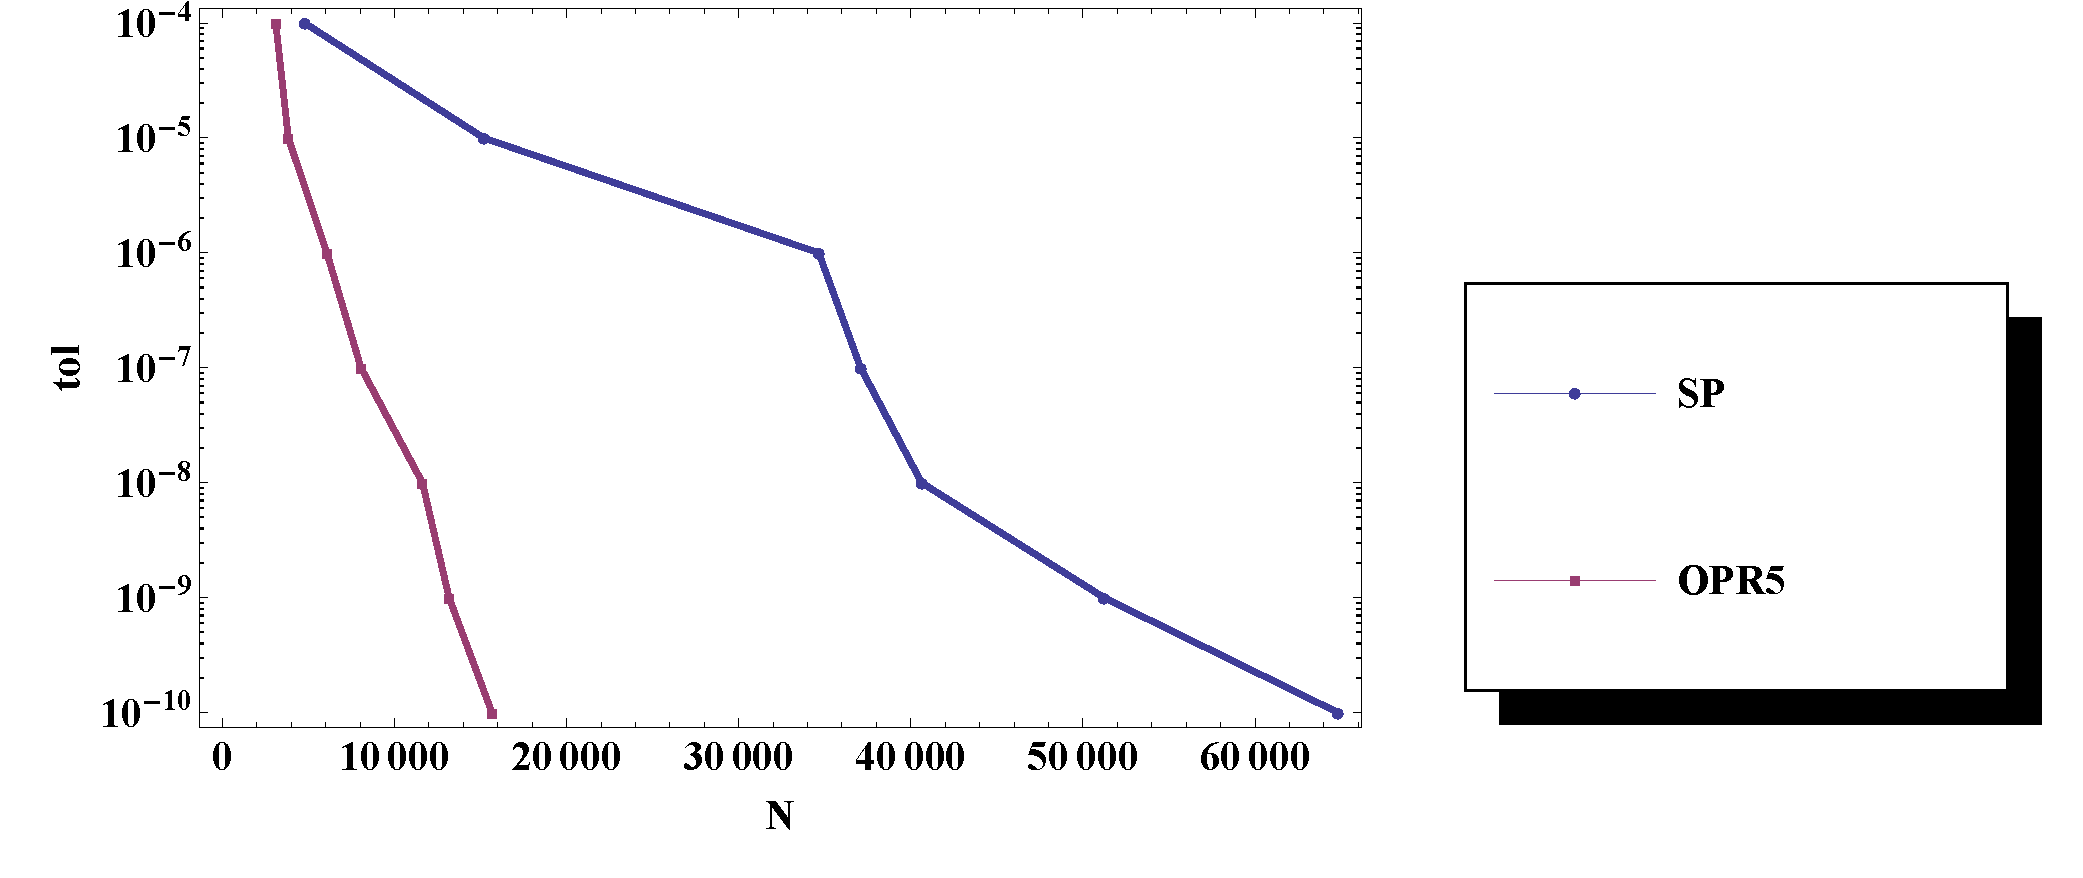
\includegraphics[height=6cm]{num_ex_1_1.pdf}
% \caption{\small Возрастание времени выполнения с увеличением размерности  }
% \label{num_ex_1_1}
% \end{figure}

% Положим теперь $N = 885$, оставляя остальные параметры численного эксперимента неизменными, и исследуем время решения каждым из приведенных алгоритмов при постепенном увеличении шага $\tau$

% \begin{figure}[H]
% 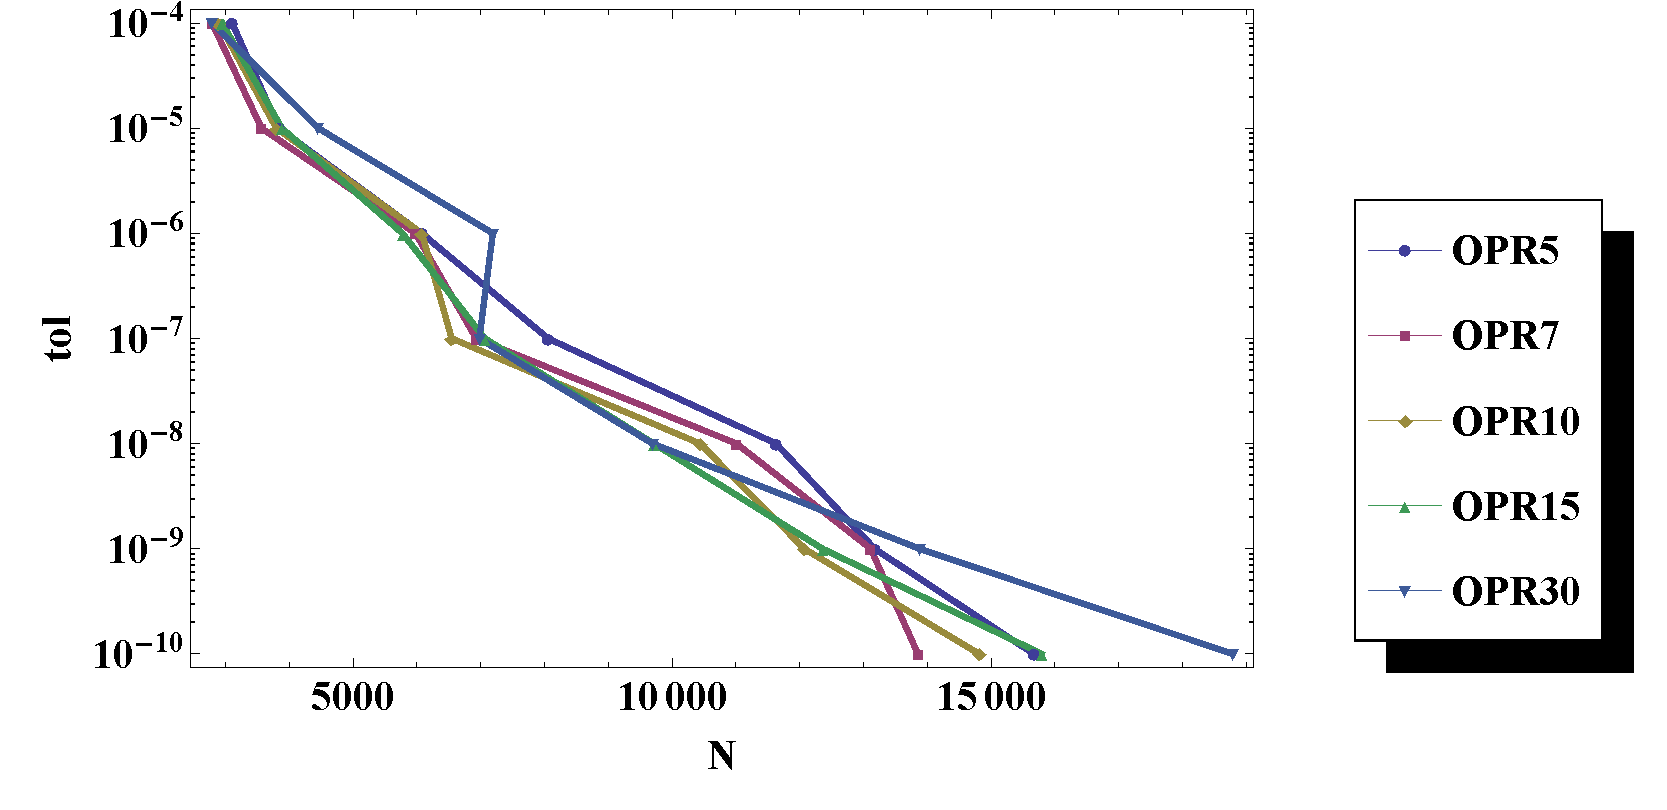
\includegraphics[height=6cm]{num_ex_1_2.pdf}
% \caption{\small Изменение трудоемкости с увеличением шага $\tau$ с 5 до 25}
% \label{num_ex_1_2}
% \end{figure}

% Следующий эксперимент демонстрирует влияние величины разброса собственных значений на скорость сходимости итерационных процессов: зафиксировав $N=531$, $\tau = 10$, $\rho_{min}=1$, будем изменять $\rho_{max}$ от $10$ до $10^{3}$. Результат представлен на рисунке \ref{num_ex_1_3}.

% \begin{figure}[H]
% 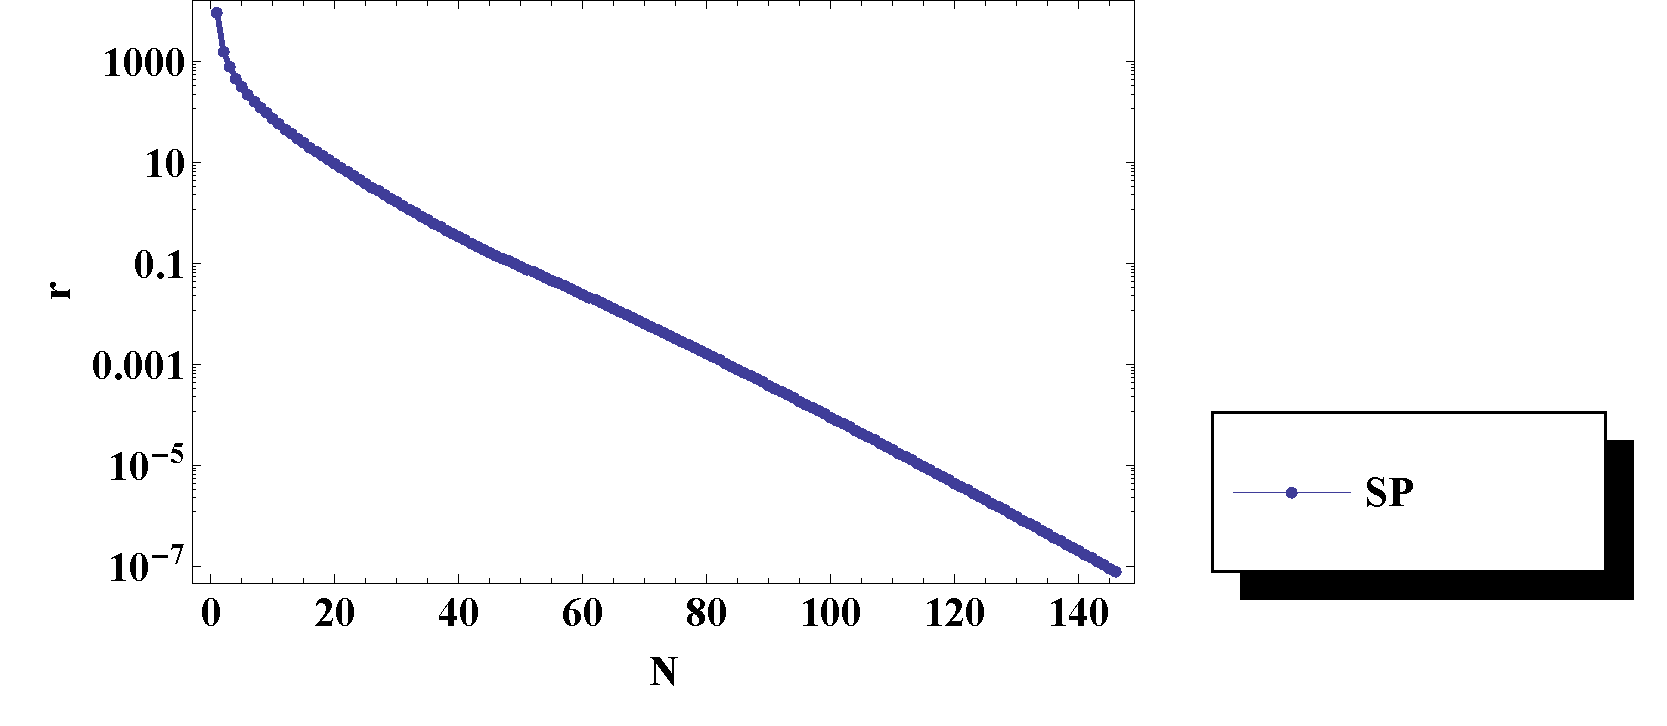
\includegraphics[height=6cm]{num_ex_1_3.pdf}
% \caption{\small Изменение трудоемкости с увеличением  $\rho_{max}$ c $10$ до $10^4$}
% \label{num_ex_1_3}
% \end{figure}

% Аналогично предыдущему случаю, исследуем влияние изменения $\rho_{min}$ на скорость сходимости. Для этого зафиксируем $N=531$, $\tau = 10$, $\rho_{max}=100$ и будем изменять $\rho_{min}$ в диапазоне от $10^{-4}$. Графики зависимости времени работы от $\rho_{min}$ на рисунке \ref{num_ex_1_4}.

% \begin{figure}[H]
% 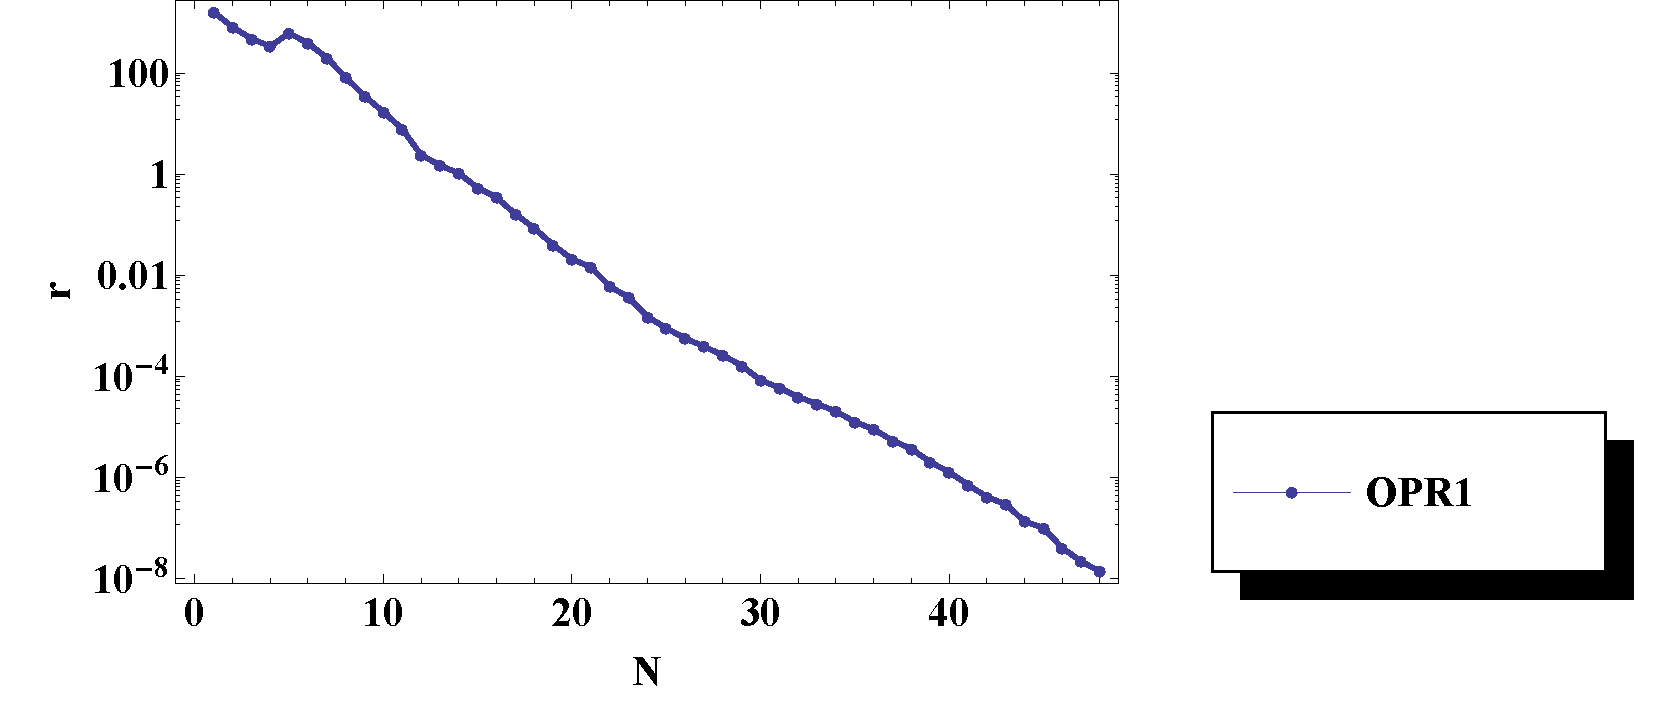
\includegraphics[height=7cm]{num_ex_1_4.pdf}
% \caption{\small Изменение трудоемкости с увеличением  $\rho_{min}$ c $10^{-4}$ до $1$}
% \label{num_ex_1_4}
% \end{figure}

% Следующая серия экспериментов будет проведена с углом $\alpha = \frac{\pi}{3}$.

\section{Задача с собственными значениями из сектора}
 Для первого эксперимента мы взяли область распределения собственных значений как сектор кольца с минимальным и максимальным радиусом $\rho_{min}=1$ и $\rho_{max} = 300$ соответственно, $\alpha = \frac{\pi}{3}$ (рисунок \ref{region_evals}).  Начальные условия $y_0=(1,...,1)$, функция правой части константная, $f(t) = (5,...,5)$. Матрицы $J$ генерируются следующим образом: сначала на диагональ матрицы устанавливаются блоки, соответствующие комплексно-сопряженным парам собственных значений, а затем применяем преобразование отражения. Таким образом, матрицы являются полными. Также стоит отметить, что если матрица исходной системы имеет размерность $M$, то после применения неявного метода размерность задачи составит уже $N = s\ M$, где $s$ - число стадий базового метода (во всех наших экспериментах оно равно 3). Далее под $N $ будет подразумеваться размерность матрицы $G$.

\begin{figure}[H]
\begin{center}
\includegraphics[height=10cm]{region.pdf}
\caption{\small Область распределения собственных значений матрицы $J$}
\label{region_evals}
\end{center}
\end{figure}

Отследим эффективность различных алгоритмов при изменении только размерности, не затрагивая при этом основных спектральных характеристик  $\rho_{min}$ и $\rho_{max}$. Параметры эксперимента следующие: $\rho_{max} = 100$, $\rho_{min} = 1$, $\tau = 10$. Дополнительно для сравнения мы привели результаты метода, чья область устойчивости является сектором с углом $\alpha=\frac{\pi}{3}$. Результаты для  не переобусловленного и переобусловленного случаев представлены на рисунках  \ref{num_ex_2_1n} и  \ref{num_ex_2_1p} соответственно.
\begin{figure}[H]
\includegraphics[height=6cm]{num_ex_2_1n.pdf}
\caption{\small Изменение трудоемкости с увеличением  $N$ (без переобусловливания)}
\label{num_ex_2_1n}
\end{figure}
\begin{figure}[H]
\includegraphics[height=6cm]{num_ex_2_1p.pdf}
\caption{\small Изменение трудоемкости с увеличением  $N$ (с переобусловливанием)}
\label{num_ex_2_1p}
\end{figure}

Положим теперь $N = 885$, оставляя остальные параметры численного эксперимента неизменными, и исследуем время решения каждым из приведенных алгоритмов при постепенном увеличении шага $\tau$ в случае с переобусловливанием (рис. \ref{num_ex_2_2p}) и без него (рис. \ref{num_ex_2_2n}).

\begin{figure}[H]
\includegraphics[height=6cm]{num_ex_2_2p.pdf}
\caption{\small Изменение трудоемкости с увеличением шага $\tau$ с 5 до 30 (с переобусловливанием)}
\label{num_ex_2_2p}
\end{figure}

\begin{figure}[H]
\includegraphics[height=6cm]{num_ex_2_2n.pdf}
\caption{\small Изменение трудоемкости с увеличением шага $\tau$ с 5 до 30 (без переобусловливания) }
\label{num_ex_2_2n}
\end{figure}


Следующий эксперимент демонстрирует влияние величины разброса собственных значений на скорость сходимости итерационных процессов: зафиксировав $N=885$, $\tau = 10$, $\rho_{min}=1$, будем изменять $\rho_{max}$ от $10$ до $10^{3}$. Результат представлен на рисунка \ref{num_ex_2_4p} и \ref{num_ex_2_4n}.

\begin{figure}[H]
\includegraphics[height=6cm]{num_ex_2_4p.pdf}
\caption{\small Изменение трудоемкости с увеличением  $\rho_{max}$ c $10$ до $10^3$ (с переобусловливанием)}
\label{num_ex_2_4p}
\end{figure}

\begin{figure}[H]
\includegraphics[height=6cm]{num_ex_2_4n.pdf}
\caption{\small Изменение трудоемкости с увеличением  $\rho_{max}$ c $10$ до $10^3$ (без переобусловливания)}
\label{num_ex_2_4n}
\end{figure}

Исследуем влияние изменения $\rho_{min}$ на скорость сходимости. Для этого зафиксируем $N=531$, $\tau = 10$, $\rho_{max}=100$ и будем изменять $\rho_{min}$ в диапазоне от $10^{-4}$. Графики зависимости времени работы от $\rho_{min}$ на рисунках \ref{num_ex_2_3p} и \ref{num_ex_2_3n}.

\begin{figure}[H]
\includegraphics[height=7cm]{num_ex_2_3p.pdf}
\caption{\small Изменение трудоемкости с увеличением  $\rho_{min}$ c $10^{-3}$ до $1$ (с переобусловливанием)}
\label{num_ex_2_3p}
\end{figure}

\begin{figure}[H]
\includegraphics[height=7cm]{num_ex_2_3n.pdf}
\caption{\small Изменение трудоемкости с увеличением  $\rho_{min}$ c $10^{-3}$ до $1$ (без переобусловоивания)}
\label{num_ex_2_3n}
\end{figure}

Приведём также графики (рисунки \ref{num_exp_5_3p}  и  \ref{num_exp_5_3n}) скорости решения системы с $\rho_{min}=1$ и $\rho_{max}=10$ и $\tau = 10$. $N$ изменяется в пределах от 354 до 4602.

\begin{figure}[H]
\includegraphics[height=7cm]{num_ex_5_4p.pdf}
\caption{\small Изменение трудоемкости с увеличением  $N$ c 354 до 4602 (с переобусловливанием)}
\label{num_exp_5_3p}
\end{figure}

\begin{figure}[H]
\includegraphics[height=7cm]{num_ex_5_4n.pdf}
\caption{\small Изменение трудоемкости с увеличением  $N$ c 354 до 4602 (без переобусловоивания)}
\label{num_exp_5_3n}
\end{figure}

Исследуем влияние изменения шага по времени для задачи с малым отношением $\frac{\rho_{min}}{\rho_{max}}$. Параметры следующие: $\rho_{min}=1000$, $\rho_{max}=2000$, $\tau  = 10$. Результаты представлены на рисунках \ref{num_exp_6_1p} и \ref{num_exp_6_1n}
\begin{figure}[H]
\includegraphics[height=7cm]{num_ex_6_1p.pdf}
\caption{\small Изменение трудоемкости с увеличением  $\tau$ c 0.1 до  c 0.1 до $10^{5}$ (с переобусловливанием)}
\label{num_exp_6_1p}
\end{figure}

\begin{figure}[H]
\includegraphics[height=7cm]{num_ex_6_1n.pdf}
\caption{\small Изменение трудоемкости с увеличением  $\tau$ c 0.1 до $10^{5}$ (без переобусловливания)}
\label{num_exp_6_1n}
\end{figure}

Таким образом можно заключить, что чем ближе $\rho_{min}$ к $ \rho_{max}$, тем быстрее работают методы, причем изменение шага $\tau$ фактически не влияет на трудоемкость отыскания решения, что в свою очередь, является очень полезным свойством при решении жёстких задач.


\section{Случай наличия близких к нолю действительных частей собственных значений}

Предыдущие эксперименты демонстрировали превосходство методов GMRES
и BIСGSTAB над разрабатываемым. Однако, в случае,когда собственные
значения матрицы $J$ находятся вблизи мнимой оси (в данном
эксперименте это величины поряка $10^{-5}$, см. рис. \ref{bad_for_gmres}),
получается кардинально иная картина. На графике скорость работы
метода BIСGSTAB не отражена, поскольку этот метод вообще не
сходится.

\begin{figure}[H]
\begin{center}
\includegraphics[height=6cm]{bad_for_gmres.pdf}
\caption{\small Собственные значения матрицы $J$. $N = 236$}
\label{bad_for_gmres}
\end{center}
\end{figure}

Чтобы это продемонстрировать, зададим параметры эксперимента
следующим образом: $\tau = 10$, $\rho_{min} = 1$, $\rho_{max} = 300$
и будем увеличивать $N$. Результаты представлены на рисунке
\ref{num_ex_3_1}.

\begin{figure}[H]
\includegraphics[height=7cm]{num_ex_3_1.pdf}
\caption{\small Изменение трудоемкости с увеличением $N$ c 354 до 1062}
\label{num_ex_3_1}
\end{figure}

Стоит отметить, что метод GMRES на задаче с $N=1062$ сходится более чем за 2700 секунд, но точное время работы было решено не устанавливать поскольку даже этот результат достаточно характеризует картину.

\section{Линейная задача с разреженной матрицей}

Матрица у представленных выше задач являлась полной. Рассмотрим теперь задачу с ленточной матрицей. Положим
$$ y'(t)=J y(t) + f(t), \quad t\in[0,0.15], \quad M\in \mathbb R^N\times \mathbb R^N,$$
$$f_i = t \exp (10 t),$$
$$y(0) = (1,...,1)^T,$$

$$J =
\left(
\begin{array}{ccccc}
-3&1&0& &0\\
-4&-12&4& &\\
&\ddots&\ddots&\ddots\\
& & -(N-1)^2&-3(N-1)^2&(N-1)^2\\
0& & &-N^2&-3N^2
\end{array}\right).$$
Спектр матрицы $J$ этой задачи при различных $N$ представлен на рисунке \ref{j_spektrum_3_exp}. Учитывая область распределения собственных значений, можно воспользоваться методом с областью устойчивости в секторе с углом $\frac{\pi}{3}$. Шаг по времени  $\tau = 0.15$. Результаты работы представлены на рисунках  \ref{exp_3_1p} и \ref{exp_3_1n}.

\begin{figure}[H]
\begin{tabular}{cc}
\includegraphics[height=4cm]{3_spektr50.pdf}& \includegraphics[height=4cm]{3_spektr100.pdf}
\end{tabular}
\caption{\small Спектр матрицы $J$ для $N = 50$  и $N = 100$}
\label{j_spektrum_3_exp}
\end{figure}

\begin{figure}[H]
\includegraphics[height=7cm]{num_ex_4_1p.pdf}
\caption{\small Зависимость времени работы от размерности $N$. Случай с переобусловливанием.}
\label{exp_3_1p}
\end{figure}

\begin{figure}[H]
\includegraphics[height=7cm]{num_ex_4_1n.pdf}
\caption{\small Зависимость времени работы от размерности $N$. Случай  без переобусловливания.}
\label{exp_3_1n}
\end{figure}

На графике \ref{exp_3_1p} отражены данные только для $N$ от 300 до 900, поскольку даже при 900 вычисления занимают около 20 минут и при увеличении размерности это время ещё возрастет.

\newpage
\likechapter{ЗАКЛЮЧЕНИЕ}

 В работе представлен подход к реализации неявных методов для жёстких систем с на основе метода установления. Приведены расчётные формулы и данные численного эксперимента.

Рассмотрена и реализована возможность расширения области
применимости методов, основанных на принципе установления при помощи
переобусловливания.

Разработанный метод применен для решения  тестовых линейных задач с
заданным спектром. По результатам можно сказать, что разработанный
метод подходит для решения задач со спектром из левой комплексной
полуплоскости, причем в отдельных случаях работает лучше чем
некоторые известные методы. При этом стоит особо отметить, что
предлагаемые итерационные процессы естественным образом применимы в
нелинейном случае, тогда как <<решатели>> GMRES и BICGSTAB --- нет.

Низкая эффективность  метода некоторых тестовых задачах может быть
объяснена следующим образом: во-первых, в силу технических
ограничений расчеты производились на матрицах относительно небольшой
размерности, во-вторых реализация метода может быть не самой
оптимальной.
% Выводы:
% \begin{enumerate}
% \item Для реализации схем относительно небольшим количеством уравнений применять принцип установления нецелесообразно.
% \item Если количество уравнений в системе велико, то методы основанные на идее установления работают эффективнее и потребляют меньшее количество вычислительных ресурсов.
% \end{enumerate}


\newpage

\begin{thebibliography}{99}
\bibitem{dekker}Деккер К., Вервер Я. Устойчивость методов Рунге—Кутты для жестких нелинейных дифференциальных уравнений/ Пер. с англ.— М.: Мир, 1988.

\bibitem{Faleichik_Bondar_Kyiv}Фалейчик Б. В., Бондарь И. В. Реализация неявных методов для жестких задач методом установления// Theoretical and Applied Aspects of Cybernetics. Proceedings of the International Scientific Conference of Students and Young Scientists -- Kyiv: Bukrek, 2011. С. 297-299.

\bibitem{Faleichik_article}Faleichik B. V. Explicit Implementation of Collocation Methods for Stiff Systems with Complex Spectrum // Journal of Numerical Analysis, Industrial and Applied Mathematics. Vol. 5

\bibitem{Faleichik_bondar_amade}Фалейчик Б. В., Бондарь И. В. Реализация неявных методов Рунге-Кутты с использованием принципа установления //Аналитические методы анализа и дифференциальных уравнений: Тез. докл. междунар. конф. 12-17 сент. 2011г, Минск, Беларусь. С. 146-147

\bibitem{hairer}Хайрер Э., Ваннер Г.  Решение обыкновенных дифференциальных уравнений. Жесткие и дифференциально-алгебраические задачи./ Пер. с англ. — М.: Мир, 1999. — 685 с.

\bibitem{Faleichik_amade}Фалейчик Б. В. Реализация неявных методов для жестких задач с использованием обобщенных итераций Пикара // Тр. 6-й международной конференции «Аналитические методы анализа и дифференциальных уравнений»: в двух томах – Т.1 Математический анализ. — Минск: Институт математики НАН Беларуси, 2012. С. 131–135.

\bibitem{gomel}Фалейчик Б. В., Бондарь И. В. Реализация неявных методов Рунге-Кутты для больших жестких систем//Новые математические методы и компьютерные технологии в проектировании, производстве и научных исследованиях: XV Республиканская научная конференция студентов и аспирантов ``Новые математические методы и компьютерные технологии в проектировании, производстве и научных исследованиях'', 26-28 марта 2012 г.:[материалы]: в 2 ч. Ч.1/редкол. : Демиденко О.М. -- Гомель: ГГУ им. Ф. Скорины, 2012. С. 175-176
\bibitem{konf_may}Бондарь И. В. Итерационные процессы установления для жестких линейных задач //Тр. 69-й ежегодной научной конференции студентов и аспирантов БГУ: допущено в печать.

\bibitem{deal} Интернет адрес: http://www.dealii.org
\end{thebibliography}

\end{document}
